% Format teze zasnovan je na paketu memoir
% http://tug.ctan.org/macros/latex/contrib/memoir/memman.pdf ili
% http://texdoc.net/texmf-dist/doc/latex/memoir/memman.pdf
% 
% Prilikom zadavanja klase memoir, navedenim opcijama se podešava 
% veličina slova (12pt) i jednostrano štampanje (oneside).
% Ove parametre možete menjati samo ako pravite nezvanične verzije
% mastera za privatnu upotrebu (na primer, u b5 varijanti ima smisla 
% smanjiti 
\documentclass[12pt,oneside]{memoir} 

% Paket koji definiše sve specifičnosti master rada Matematičkog fakulteta
\usepackage[latinica]{matfmaster} 
%
% Podrazumevano pismo je ćirilica.
%   Ako koristite pdflatex, a ne xetex, sav latinički tekst na srpskom jeziku
%   treba biti okružen sa \lat{...} ili \begin{latinica}...\end{latinica}.
%
% Opcija [latinica]:
%   ako želite da pišete latiniciom, dodajte opciju "latinica" tj.
%   prethodni paket uključite pomoću: \usepackage[latinica]{matfmaster}.
%   Ako koristite pdflatex, a ne xetex, sav ćirilički tekst treba biti
%   okružen sa \cir{...} ili \begin{cirilica}...\end{cirilica}.
%
% Opcija [biblatex]:
%   ako želite da koristite reference na više jezika i umesto paketa
%   bibtex da koristite BibLaTeX/Biber, dodajte opciju "biblatex" tj.
%   prethodni paket uključite pomoću: \usepackage[biblatex]{matfmaster}
%
% Opcija [b5paper]:
%   ako želite da napravite verziju teze u manjem (b5) formatu, navedite
%   opciju "b5paper", tj. prethodni paket uključite pomoću: 
%   \usepackage[b5paper]{matfmaster}. Tada ima smisla razmisliti o promeni
%   veličine slova (izmenom opcije 12pt na 11pt u \documentclass{memoir}).
%
% Naravno, opcije je moguće kombinovati.
% Npr. \usepackage[b5paper,biblatex]{matfmaster}

% Pomoćni paket koji generiše nasumičan tekst u kojem se javljaju sva slova
% azbuke (nema potrebe koristiti ovo u pravim disertacijama)
\usepackage[latinica]{pangrami}

% Datoteka sa literaturom u BibTex tj. BibLaTeX/Biber formatu
\bib{references}

% Ime kandidata na srpskom jeziku (u odabranom pismu)
\autor{Ivan Ristović}
% Naslov teze na srpskom jeziku (u odabranom pismu)
\naslov{Kreiranje zajedničke AST apstrakcije za različite programske jezike}
% Godina u kojoj je teza predana komisiji
\godina{2020}
% Ime i afilijacija mentora (u odabranom pismu)
\mentor{doc. dr Milena \textsc{Vujošević-Janičić}\\ Univerzitet u Beogradu, Matematički fakultet}
% Ime i afilijacija prvog člana komisije (u odabranom pismu)
\komisijaA{dr Ana \textsc{Anić}\\ University of Disneyland, Nedođija}
% Ime i afilijacija drugog člana komisije (u odabranom pismu)
\komisijaB{dr Laza \textsc{Lazić}\\ Univerzitet u Beogradu, Matematički fakultet}
% Ime i afilijacija trećeg člana komisije (opciono)
% \komisijaC{}
% Ime i afilijacija četvrtog člana komisije (opciono)
% \komisijaD{}
% Datum odbrane (odkomentarisati narednu liniju i upisati datum odbrane ako je poznat)
% \datumodbrane{}

% Apstrakt na srpskom jeziku (u odabranom pismu)
\apstr{%
\pangrami
}

% Ključne reči na srpskom jeziku (u odabranom pismu)
\kljucnereci{TODO}

\begin{document}
% ==============================================================================
% Uvodni deo teze
\frontmatter
% ==============================================================================
% Naslovna strana
\naslovna
% Strana sa podacima o mentoru i članovima komisije
\komisija
% Strana sa posvetom (u odabranom pismu)
\posveta{TODO zahvalnica}
% Strana sa podacima o disertaciji na srpskom jeziku
\apstrakt
% Sadržaj teze
\tableofcontents*

% ==============================================================================
% Glavni deo teze
\mainmatter
% ==============================================================================

\chapter{Uvod}
\label{chp:intro}

\pangrami

\section{Primeri korišćenja klasičnih \LaTeX{} elemenata}
% Primeri citiranja
Ovo je rečenica u kojoj se javlja citat \cite{PetrovicMikic2015}.
Još jedan citat \cite{GuSh:243}.
% Primeri navodnika
Isprobavamo navodnike: "Rekao je da mu se javimo sutra".
% Primer referisanja na tabelu (koja se javlja kasnije)
U tabeli \ref{tbl:rezultati} koja sledi prikazani su rezultati eksperimenta.
% Primer kraćeg ćiriličkog teksta
{\cir Ово је пример ћириличког текста који се јавља у латиничком документу.}
U ovoj rečenici se javlja jedna reč na {\cir ћирилици}.
% Primer korišćenja fusnota
Iza ove rečenice sledi fusnota.\footnote{Ovo je fusnota.}

% Primer dužeg ćirličkog teksta
\begin{cirilica}
  Ово је мало дужи блок текста исписан ћириличким писмом у оквиру
  латиничког документа. Фијуче ветар у шибљу, леди пасаже и куће иза
  њих и гунђа у оџацима.
\end{cirilica}

% Primer korišćenja tabele
\begin{table}
\centering
\caption{Rezultati}
\label{tbl:rezultati}
\begin{tabular}{c>{\centering}p{2cm}c}
\toprule
1 & 2 & 3\\\midrule
4 & 5 & 6\\\cmidrule(rl){1-2}
7 & 8 & 8\\
\bottomrule
\end{tabular}
\end{table}

% Primer korišćenja slike
\begin{figure}[!ht]
  \centering
  \label{fig:grafikon}
  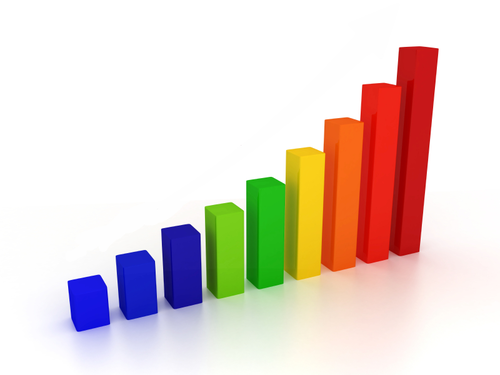
\includegraphics[width=0.5\textwidth]{images/graph.png}
  \caption{Grafikon}
\end{figure}


% Primer jednostavnije matematičke formule
Evo i jedan primer matematičke formule: $e^{i\pi} + 1 = 0$. 
% Primer referisanja na sliku
Na slici \ref{fig:grafikon} prikazan je jedan grafikon.

% primer kompleksnije matematičke formule
$$
\int_a^b f(x)\ \mathrm{d}x \ =_{def}\ \lim_{\max{\Delta x_k \rightarrow 0}} \sum_{k=1}^n f(x_k^*)\Delta x_k
$$

% primer referisanja na poglavlja i strane poglavlja
Više detalja biće dato u glavi \ref{chp:razrada} na strani \pageref{chp:razrada}.

% primer liste
Možemo praviti i nabrajanja:
\begin{enumerate}
\item Analiza 1
\item Linearna algebra
\item Analitička geometrija
\item Osnovi programiranja
\end{enumerate}

\pangrami

\chapter{Zaključak}
\label{chp:conclusion}

\pangrami

\pangrami


% ------------------------------------------------------------------------------
% Literatura
% ------------------------------------------------------------------------------
\literatura

% ==============================================================================
% Završni deo teze i prilozi
\backmatter
% ==============================================================================

% ------------------------------------------------------------------------------
% Biografija kandidata
\begin{biografija}
  \textbf{Ivan Ž. Ristović} rođen je 17.01.1995. godine u Užicu. Osnovnu školu, kao i 
  prirodno-matematički smer Užičke gimnazije, završio je kao nosilac Vukove diplome. 
  Tokom navedenog perioda školovanja isticao se u oblastima matematike, informatike, 
  fizike, hemije i engleskog jezika, što potvrđuje veći broj nagrada na Državnim 
  takmičenjima.

  Smer Informatika na Matematičkom fakultetu Univerziteta u Beogradu upisuje 2014. 
  godine. Na navedenom smeru je diplomirao 2018. godine, posle tri godine studija 
  sa prosečnom ocenom 9,17. Master studije upisuje na istom fakultetu odmah nakon 
  diplomiranja.
  
  U avgustu 2018. biva izabran u zvanje „Saradnik u nastavi“ na Matematičkom 
  fakultetu paralelno sa master studijama. Drži vežbe iz kurseva "Računarske mreže",
  "Funkcionalno programiranje", "Programske paradigme" i "Objektno orijentisano 
  programiranje" na kasnijim godinama osnovnih studija.
  
  Oblasti interesovanja uključuju pre svega razvoj i verifikaciju softvera, mikroservise 
  i računarske mreže.
\end{biografija}
% ------------------------------------------------------------------------------

\end{document}
